\documentclass[conference]{IEEEtran}
\usepackage{cite}
\usepackage[]{algorithm2e}
\usepackage{amsmath}
\usepackage{graphicx}
\usepackage{caption}
\graphicspath{ {images/} }

\begin{document}

\title{Indoor Localization for Mobile Devices Using Bluetooth Low Energy Beacons and Wi-Fi Access Points}

\author{
\IEEEauthorblockN{Justin L. Sewell, Alfredo J. Perez}
\IEEEauthorblockA{TSYS School of Computer Science\\
Columbus State University\\
Columbus, GA 31907\\
Email: sewell\_justin@columbusstate.edu\\
Email: perez\_alfredo@columbusstate.edu}
\and
\IEEEauthorblockN{Juan C. Morales}
\IEEEauthorblockA{Dept. of Computer Science\\
University of Puerto Rico in Bayamon\\
Bayamon, Puerto Rico 00959\\
Email: juan.morales5@upr.edu}
\and
\IEEEauthorblockN{Miguel Labrador}
\IEEEauthorblockA{Dept. of Computer Science\\
and Engineering\\
University of South Florida\\
Tampa, FL 33620\\
Email: mlabrador@usf.edu}}

\maketitle

\begin{abstract}
Indoor navigation systems have been in increasing demand since the introduction of smart-phone technology; however, no standard system for indoor navigation has been established. An indoor navigation system has many applications, especially for the 7.3 million visually impaired people in the United States. Due to the weaknesses of GPS and wireless signals indoors, the problem of localizing and tracking has proven to be difficult. Current approaches have utilized techniques such as fingerprinting and radio frequency progation models for localization. The best of these systems have achieved less than 2.5m at 90\% of the time. However, this accuracy must be improved for a viable indoor navigation system. This paper proposes BluNavi, a cost-efficient and widely deployable indoor navigation system. BluNavi uses two modules: Wi-Fi fingerprinting and an extended Kalman Filter based on dead reckoning and bluetooth low energy beacon signals.
\end{abstract}


\section{Introduction}
Indoor navigation systems have been in increasing demand since the introduction of smart-phone technology. The sensors in smart-phones can be used to provide accurate localization in an outdoor environment by using the Global Positioning System, but so far, no standard indoor localization system has been implemented due to inaccuracy and cost.

The problem with such a system pertains to localizing and tracking the user in an indoor space. This problem has many challenges that must be solved. Mainetti, et al. \cite{mainetti2014survey} lists some of these challenges, including: the loss of signal precision of wireless systems due to Non-Line-of-Sight (NLOS) conditions and multipath effect, scaling the system for large spaces, and complex environments.

A practical, accurate and cost-efficient indoor navigation system that solves these challenges has many beneficial applications such as assisting firemen to navigate a burning, smoke-filled building, locating people in danger in emergency situations, and navigation of public spaces such as malls, airports, and university buildings.

One important but unconsidered application of an indoor navigation system is assistance for the visually impaired. In 2013, there was a reported 7.3 million people in the United States with some form of visual impairment \cite{NFB}. With no form of eletronic navigation assistance when in an indoor setting, these individuals are hindered when traversing public spaces, such as malls, universities, airports and bus or train stations, among others. This would mean these individuals will need some form of help to locate his or her desired destination in such structures.

Many methods of indoor localization systems have been explored. Previous methods that have been tested use technologies such as GSM (the current global mobile communication standard), radio frequency identification tags (RFID), infrared beacons and receivers, and ultrasonic sensors \cite{otsason2005accurate,li2011performance,liu2014survey,ward1997new,medina2013ultrasound}. Unfortunately, none of these approaches were adopted because of different drawbacks such as short detection ranges, high installation costs, unsuitable levels of accuracy, and little space for improvement.

Other more practical solutions to the localization problem use the Wi-Fi infrastructure that is available in most buildings to reduce cost and installation times. The signal of the Wi-Fi Access Points (AP) can be used to approximate location using the Received Signal Strength Indicator (RSSI). However, These techniques alone are usually not enough to provide acceptable accuracy.

More recently, approaches that use Bluetooth Low Energy (BLE) have been tested. BLE is a technology that has recently surfaced that is used by many devices, including smart-phones. BLE beacons are a great candidate for implementing indoor localization due to their low energy consumption, compact size and affordability.

Recently, Google released Eddystone™, an open BLE beacon format that can be configured to send several different types of payloads using the same packet format \cite{Eddystone}. Before Eddystone, iBeacon, a proprietary protocol developed by Apple, was the standard format for BLE beacons. Eddystone is much more developer friendly and is becoming very popular due to its compatability with both Android and Apple mobile devices. The format can be used to create a contextually aware experience for users by delivering proximity event-triggered attachments.

Our proposed system, BluNavi, localizes the user by fusing data provided by Inertial Measurement Units (IMUs) and distance approximations calculated from BLE signals. To further increase accuracy, the system is complemented by Wi-Fi fingerprinting , a method which makes use of APs by mapping their RSSI values to absolute locations. Eddystone configured beacons will be used to drive our mobile, context based, indoor navigation application. The system will communicate with the user and the beacons/access points through an Android application to provide accurate, real-time indoor navigation. With this approach we aim to provide a low-cost, widely deployable system while still maintaining  a high-level of accuracy.

The rest of this paper is organized as follows: Section II describes current indoor localization research. Section III explains the methodology behind BluNavi and section IV contains the evaluation of the experimental results. Lastly, Section V details our conclusions and future work.


\section{Related Work}
Wi-Fi based indoor localization has been a widely researched topic due to its availability, and the recent surge of BLE beacons has also spurred an interest in applying previous methods used in Wi-Fi and other technologies to the advantages of BLE. Most of these approaches use the RSSI of the wireless signal to approximate the location of the device.

Wi-Fi Fingerprinting is a highly popular technique in indoor localization \cite{chan2012indoor,navarro2010wi}. This technique focuses on  building a signal strength map of a given area by creating reference points around it. In each of these reference points, RSSI values are gathered for each available access point found. These values are stored in a database and identified by the reference point in which they were gathered. Localization is achieved by obtaining the signal strengths of all available AP’s at the time of a scan and matching the current values to the ones in the pre-existing database. This method has many advantages due to the system being fully based on previously installed Wi-Fi APs and not inccuring any extra hardware costs. Fingerprinting also eliminates the need of using noisy wireless signals for distance approximation. In addition, algorithms such as Nearest Neighbor or the Hidden Markov Model can be applied to the current scans to improve accuracy. However, fingerprinting also has it’s shortcomings such as long scan times and similar fingerprints.

Wu, et al. \cite{wu2016improved} improves on  Wi-Fi fingerprinting. A Particle Filter (PF) is used to fuse location estimations provided by a dead reckoning model and Wi-Fi fingerprinting to provide a higher localization accuracy. The PF is initialized using a Random Sample Consensus model which filters out the outliers of the Wi-Fi fingerprinting algorithm by comparing the estimations to the dead reckoning model, thus reducing the chance of the PF initializing in the wrong location. For the fingerprinting, two methods are examined. The first is a probabilistic approach using a Gaussian distribution to approximate the distribution of RSSI values of an AP. The second approach is deterministic using a Support Vector Machine (SVM) for pattern recognition of online readings to the database values.  The reported accuracy of the approach was less than 2.9 (m) with an average error distance of 1.2 (m). This approach has good accuracy while not requiring any additional hardware, but it also requires a lengthy off-line training phase for the fingerprint database.

BLE signal fingerprinting is an alternative to Wi-Fi AP fingerprinting. Using BLE over Wi-Fi has the advantages of faster scan times and lower power consumption. Faragher, et al. \cite{faragher2015location} established a grid and probabilities were distributed into cells using a Bayesian likelihood function based on the results of a K-Nearest-Neighbor location estimation. Accuracies of less than 2.6m at 90\% of the time were reported with a deployment of 1 beacon per 30m$^2$. This accuracy is better than Wi-Fi fingerprinting and uses less power, however the  system  requires a dense deployment of beacons to achieve medium levels of accuracies.

BLE beacon fingerprinting can be combined with a radio frequency propagation model to increase the accuracy of a system \cite{zhuang2016smartphone}. The model is built by using the relationship between signal strength and distance. Because of the large levels of noise in the signal strength, the distance approximation is subject to high levels of volatility.  An outlier detection system is used along with an extended Kalman Filter (EKF) on the fingerprint and propagation model estimations to reduce noise and improve accuracy. An improved approach to building the radio map by updating the data while the system is online to reduce time of off-line training was also used by this approach. This system achieved distance estimations of less than 2.5m at 90\% of the time for a dense deployment of beacons at 1 beacon per 9m.

The previously mentioned approaches have unique solutions that have advanced indoor localization research, but can be improved. With their shortcomings in mind, an implementation that could achieve higher accuracies, with the ability to maintain these accuracies under any sort of conditions while mainting a lower need for deployment of hardware, and thus additional costs, would be a valuable step forward for indoor localization research.
%BluNavi improves on previous systems by requiring less hardware and configuration tim
\section{Methodology}

BluNavi's system is composed of two key modules: Wi-Fi fingerprinting and an extended Kalman Filter. The system uses the fingerprinting module during NLOS conditions, such as when the user is located in a room without a beacon. This module is designed to achieve broad, room-level localization, not pin point accuracy. The purpose is to reduce the cost and complexity of the system by not requiring that beacons be installed in every room of a building, but rather just the central corridors and walkways. The second module, the extended Kalman Filter, will be used during line of sight conditions, such as when the user is traversing a hallway where beacons are deployed. The extended Kalman Filter has two sub-components: a dead reckoning model to track orientation and movement, and a propagation model to approximate distance to a BLE beacon. The filter produces a state estimate that tracks the coordinates and orientation of the user. The system diagram can be seen in Fig. \ref{fig:sysdiagram}.

\begin{figure}[h]
\centering
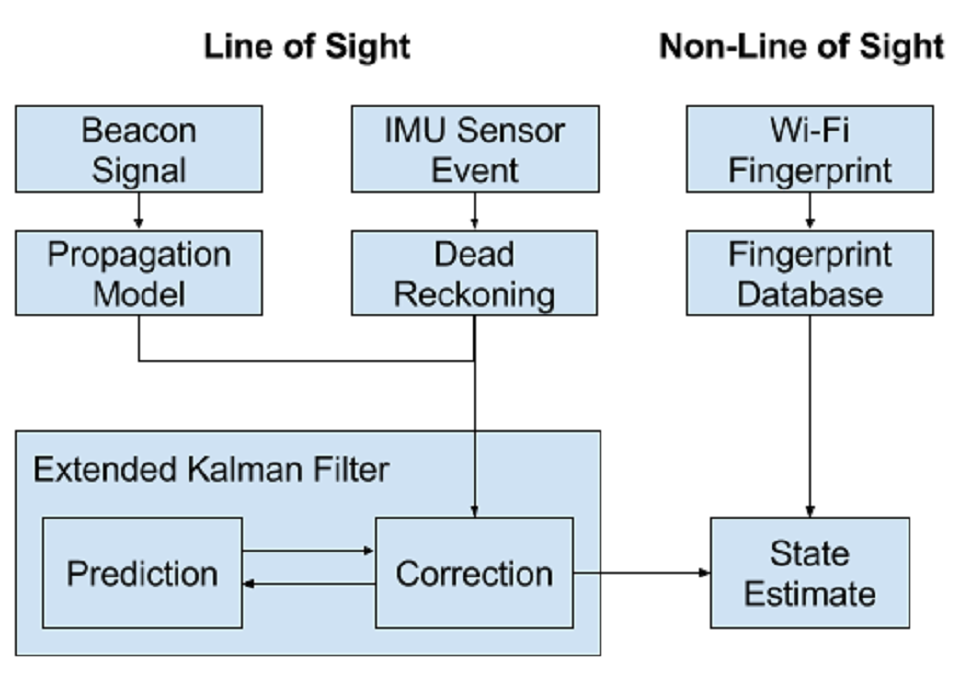
\includegraphics[scale=0.25]{SystemDiagram.png}
\caption{System Diagram}
\captionsetup{justification=centering,margin=2cm}
\label{fig:sysdiagram}
\end{figure}


\subsection{Fingerprinting}
The Wi-Fi Fingerprinting module will be used when NLOS conditions are detected from all available beacons, or when no beacons are in range of detection.
For a fingerprinting implementation, a reference point map needs to be created. At every reference point, RSSI data for every available access point needs to be collected. This is done using the following algorithm when scanning with a device.

\newcommand{\forcond}{$i=0$ \KwTo $N$}
\newcommand{\forAP}{each available AP}
\begin{algorithm}
 \KwData{Wi-Fi Scans Data}
 \KwResult{Fingerprint Database}
 \For{\forcond}{
    scan for access points\;
    \For{\forAP}{
      store AP's MAC address\;
      store AP's RSSI\;
      store current reference point\;
    }
 }
 \caption{Creating Fingerprint Database}
\end{algorithm}

Where $N$ is the amount of scans to be done. After this database is created, the system can then estimate the user’s location through a weight based approach, where a weight is assigned to each reference point based on the similarities between the user’s current scans and the fingerprint database. This is done through the following algorithm:

\newcommand{\forDB}{each ref. point containing the AP}
\begin{algorithm}
 \KwData{Wi-Fi Scans Data}
 \KwResult{User Location}
scan for access points\;
\For{\forcond}{
  \For{\forDB}{
    \If{$X < (RSSI_{AP} - RSSI_{DB}) < X$}{
      increase weight of location\;
      }
  }
 }
 \Return highest weight location\;

 \caption{Estimating User Location}
\end{algorithm}

Where $X$ is a threshold due to how RSSI values vary.

\subsection{Pedestrian Dead Reckoning Model}
BluNavi uses a Dead Reckoning (DR) model to track two key localization components: orientation and displacement (movement). Displacement occurs when the user of the system takes a step. Changes in orientation result from the user turning to face a new direction. The IMU's available in most mobile devices are used to track both components. A gyroscope is used to track changes in orientation.

Displacement of the user is estimated by calculating the length of the current step. BluNavi's DR model uses measurements provided by an accelerometer to calculate step length. The data is passed through a low-pass filter to remove noise and smooth the curve. The filtered values are then used in the formula presented by Bao, et al. \cite{bao2013indoor} which is shown by the following equation:
\begin{equation}
\label{equa:steplength}
s_n = K\sqrt[4]{a_h - a_l}
\end{equation}
where $n$ is the current step, $s_n$ is the length of step $n$, and $a_h$ and $a_l$ are the high (maximum) and low (minimum) values of the accelerometer's vertical axis during step $n$, respectively. $K$ is a constant that expresses the leg length of the user and is determined through training.

Step length is estimated upon completion of a step. Two methods can be used to determine when a step has been completed. If a step detector is available in the mobile device, then the data provided from it is used for step detection. Otherwise, a step detection process begins when the vertical acceleration values pass a set threshold. The threshold is used to avoid recording a false peak during the begining of a step. Fig. \ref{fig:accgraph} demonstrates a threshold on accelerometer data that was collected from a test where ten steps were taken. The peak is recorded when the partial derivative of the data changes from positive to negative. Then, the lowest value is recorded. When the next peak is detected, the process is over and the step length is calculated.

\begin{figure}[h]
\centering
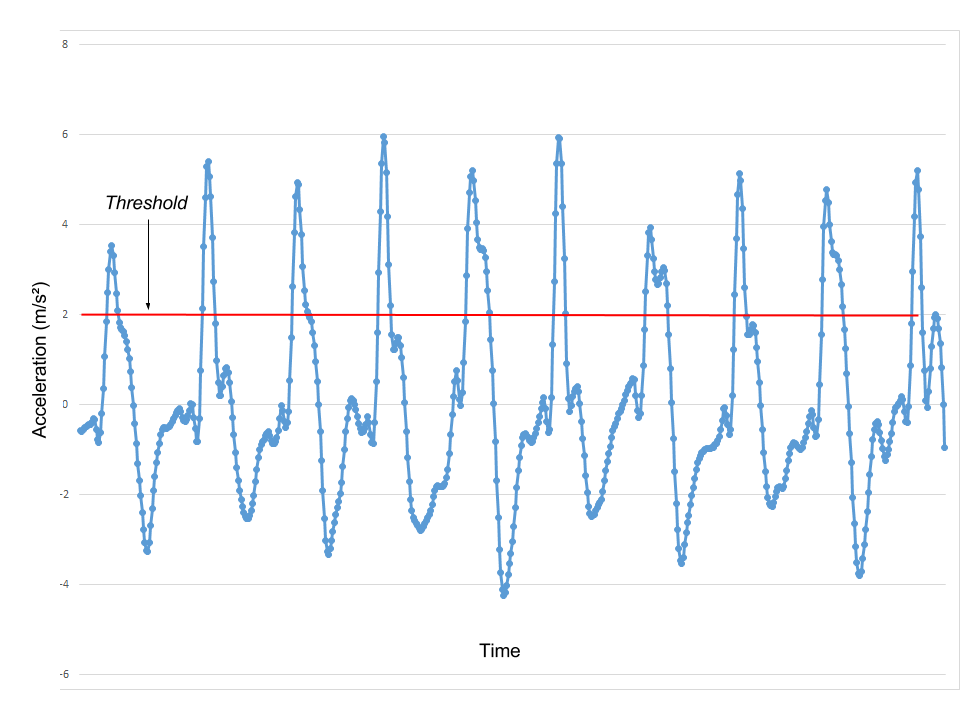
\includegraphics[scale=0.25]{AccelerometerGraph.png}
\caption{Vertical Acceleration Data}
\captionsetup{justification=centering,margin=2cm}
\label{fig:accgraph}
\end{figure}

\subsection{Propagation Model}
For indoor localization, distance from device to beacon is approximated using a radio frequency propagation model. BluNavi uses the log-distance path loss model. The model can be seen in Eq. \ref{equa:propmodel}
\begin{equation}
\label{equa:propmodel}
P(d) = P(d_0) - 10{\gamma}log_{10}(d) + X_\sigma
\end{equation}
where $P(d)$ represents the RSS at distance $d$, $P(d_0)$ is the transmit power, $\gamma$ is the path-loss exponent, and $X_\sigma$ is a Gaussian random variable with zero mean. The model has acceptable accuracy in open, line of sight environments but suffers when used in enclosed places. For this reason, an extended Kalman Filter is used to increase the accuracy.
% Distance is calculated by rewritting Eq. \ref{equa:propmodel} into Eq. \ref{equa:solvedpropmodel}.
% \begin{equation}
% \label{equa:solvedpropmodel}
% d = 10^\frac{X_\sigma + P(d_0) - P(d)}{10\gamma}
% \end{equation}

\subsection{Extended Kalman Filter}
The extended Kalman Filter (EKF) is used in BluNavi to increase the localization accuracy of the system by fusing sensor data provided by the dead reckoning model and the propagation model. The filter works in two steps: a prediction step and a correction step.

The prediction step predicts the current state and the error of the prediction using a standard Kalman Filter process model and process covariance model. The process model estimates movement (or non-movement) through the indoor environment. The model is given by Eq. \ref{equa:processmodel}
\begin{equation}
\label{equa:processmodel}
x_{kp} = Ax_{k-1} + w_k
\end{equation}
where $x_{kp}$ is the predicted state vector at time $k$, $A$ is the state transition matrix, $x_{k-1}$ is the previous state vector, and $w_k$ is zero-mean, Gaussian white-noise caused by the error in the process. The state vector is defined as \ref{equa:statevector}:
\begin{equation}
\label{equa:statevector}
x =
\begin{bmatrix}
  X & dX & Y & dY & \theta
\end{bmatrix}^T
\end{equation}
% \begin{equation}
% \label{equa:transitionmatrix}
% A =
% \begin{bmatrix}
% 1 & {\Delta}t & 0 & 0 & 0 \\
% 0 & 1 & 0 & 0 & 0 \\
% 0 & 0 & 1 & {\Delta}t & 0 \\
% 0 & 0 & 0 & 1 & 0 \\
% 0 & 0 & 0 & 0 & 1
% \end{bmatrix}
% \end{equation}
the process covariance model is defined as:
\begin{equation}
P_{kp} = AP_{k-1}A^T + Q_k
\end{equation}
where $P_{kp}$ is the predicted process covariance matrix and $Q_k$ is the process noise covariance matrix, derived from $w_k$.

Next, after sensor data is collected, a measurement model is used to record the observations:
\begin{equation}
z_k = H_kx_{k} + v_k
\end{equation}
where $z_k$ is the measurement vector, $H_k$ is the measurement transition matrix and $v_K$ is zero-mean, Gaussian white-noise caused by errors in the sensors.

The next step is to update the state vector and process covariance matrix based on the process and measurement models. The models for the step can be defined as follows:
\begin{equation}
K_k = P_{kp}H_k^T(H_kP_{kp}H_k^T + R)^{-1}
\end{equation}
\begin{equation}
x_k = x_{kp} + K_k(z_k - H_kx_{kp})
\end{equation}
\begin{equation}
P_k = (I - K_kH_k)P_{kp}
\end{equation}
where $K_k$ is the kalman gain, $R$ is the measurement noise covariance matrix dervied from $v_k$, $x_k$ is the corrected current state estimate, and $I$ is the identity matrix.



\section*{Acknowledgment}
This research has been partially supported by the National Science Foundation.


\bibliographystyle{IEEEtran}
\bibliography{bibliography}
\end{document}
